\section{Design Model}
\label{sec:Design Model}
% 
\subsection{Systemkomponenten}
\label{subsec:Systemkomponenten}
% 
\begin{figure}[H]
    \centering
    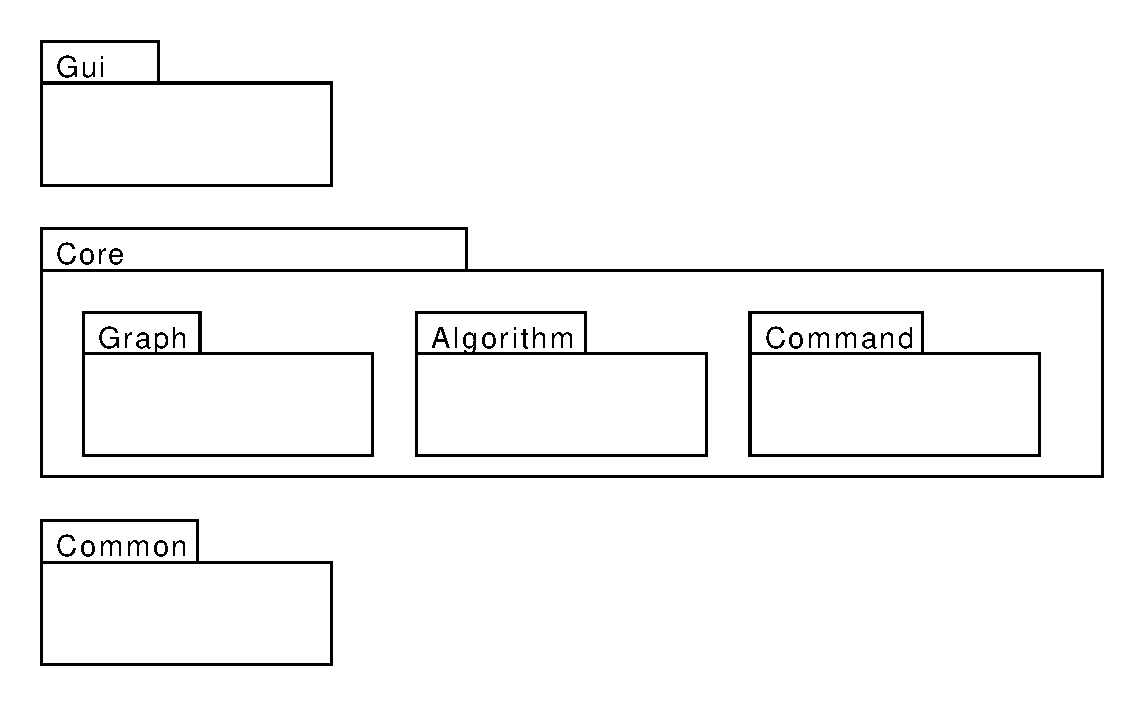
\includegraphics[scale=0.5]{diagrams/package-diagram.pdf}
    \caption{Software Architecture, Package Diagram}
    \label{fig:package-diagram}
\end{figure}
% 
Die Systemkomponenten sind in Schichten unterteilt, wobei nur eine h\"oher liegende Schicht direkten Zugriff auf eine darunterliegende Schicht hat (Schichtenarchitektur). F\"ur die Architektur lassen sich von (unten nach oben) grob die Systemkomponenten \textit{Common}, \textit{Core} und \textit{Gui} identifizieren. Die Drei-Schichten-Architektur ergibt sich aus den Requirements:
\begin{itemize}
  \item Die Komponente Common h\"alt die Interfaces f\"ur einen Actor 'Algorithm Developer' (offstage) bereit,
  \item die Komponente Gui enth\"alt die (grafische) Benutzerschnittstelle und 
  \item die Komponente Core k\"ummert sich um das Initialisieren s\"amtlicher Komponenten, I/O, Verwaltung der Parameter sowie der Berechnung der Traversierung.
\end{itemize}
% 
\begin{figure}[H]
    \centering
    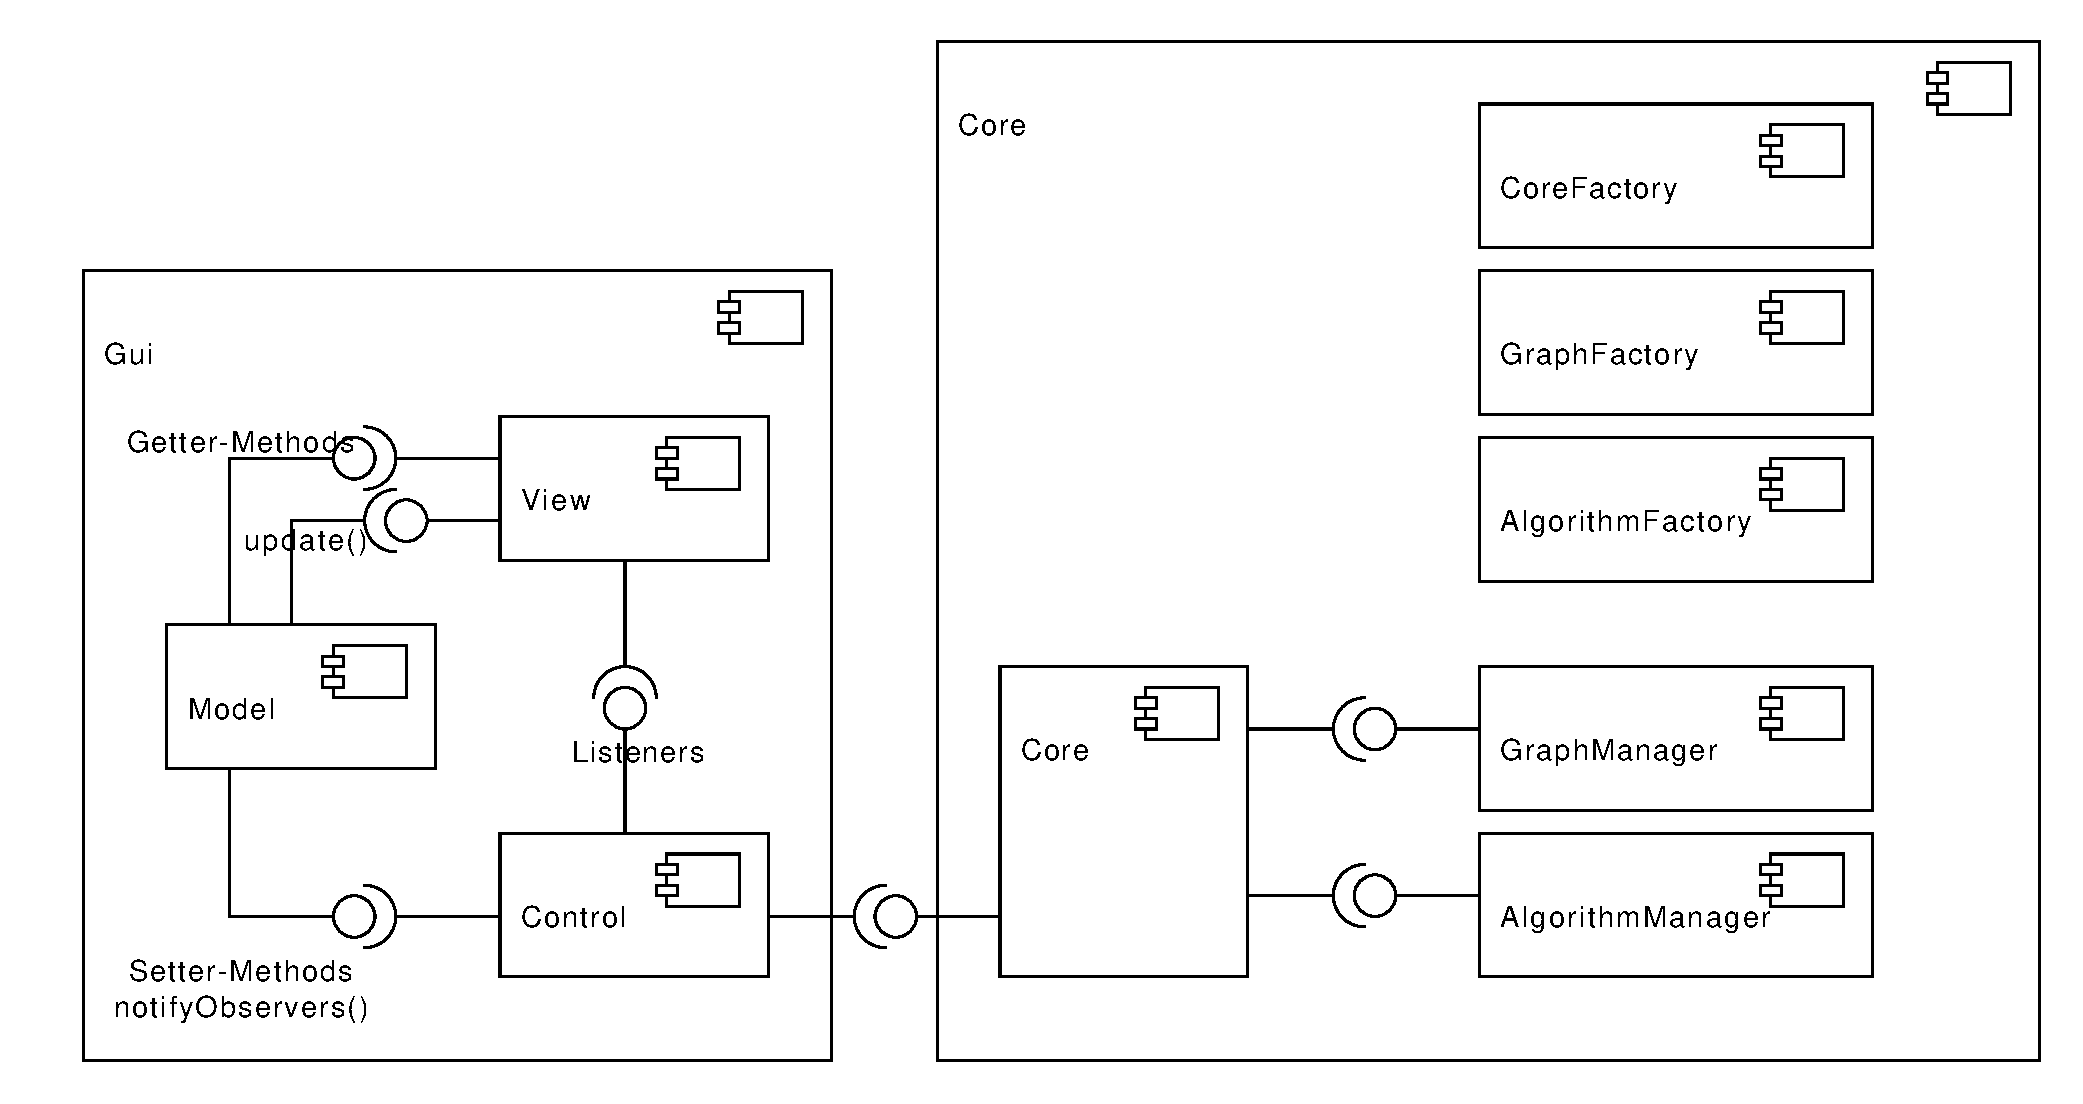
\includegraphics[scale=0.5]{diagrams/component-diagram.pdf}
    \caption{Software Architecture, Component Diagram}
    \label{fig:component-diagram}
\end{figure}
% 
\subsubsection{Common}
\label{subsubsec:Common}
Die Komponente h\"alt die f\"ur die Implementation eines Algorithmus zu verwendende Schnittstellen bereit. Diese sind f\"ur Algorithmen zu verwenden, welche importiert werden wollen.
% 
\subsubsection{Core}
\label{subsubsec:Core}
Die Komponente implementiert:
\begin{itemize}
  \item Data Model: Datenhaltung f\"ur Graph (Datenelemente Knoten und Kanten), Algorithmus und berechnete Traversierung, Traversierungsschritte als Resultat der Operation eines Algorithmus auf einen Graphen
  \item Business Logik: 
  \begin{itemize}
      \item Handling von Daten-Import und L\"oschen von Daten
      \item Validierung Graphen und Algorithmen beim Import
      \item Handling von Graphen und Algorithmen
      \item Traversierung und damit Erstellen der visualisierbaren L\"osung
  \end{itemize}
  \item Core Inteface: eine Schnittstelle, welche der Komponente GUI zur Verf\"ugung steht
\end{itemize}
% 
\subsubsection{Gui}
\label{subsubsec:Gui}
Die Komponente implementiert ein Model-View-Control (MVC) unter Verwendung des Java-Observer-Pattern:
\begin{itemize}
  \item Model: Observable mit Attributen und deren getter- und setter-Methoden
  \item View: Observer mit grafischen Elementen wie z.B. Menubar, Kn\"opfe, Regler und Text-Panelen
  \item Control: Implementiert Listeners mit deren Methoden und evtl. private Methoden
\end{itemize}
% 
\subsection{Elaboration}
\label{subsec:Elaboration}
Zur Elaboration des Designs werden die sechs Use Cases \textit{Import Graph}, \textit{Import Algorithm}, \textit{Delete Graph}, \textit{Delete Algorithm}, \textit{Select Graph} und \textit{Select Algorithm} erarbeitet und je mit einem System Sequence Diagram (SSD), einem Sequence Diagram (SD) und einem Design Class Diagram (DCD) illustriert.
\begin{itemize}
  \item Ein System Sequence Diagram zeigt, wie eine Benutzerinteraktion vom System verarbeitet wird.
  \item Ein Sequence Diagram zeigt, wie Objekte miteinander arbeiten und erl\"autert die Zust\"andigkeiten der Klassen. 
  \item Ein Design Class Diagram zeigt die Elemente des Systems unter Ber\"ucksichtigung ihrer Funktionalit\"at.
\end{itemize}

F\"ur die Use Cases \textit{Select Graph} und \textit{Select Algorithm} wird zudem die Konzeptklasse \textit{Traversal Controller} als State Machine (SM) betrachtet und mit einem State Diagram illustriert.

Ein weiteres State Diagram zeigt die Konzeptklasse \textit{Parameter Controller} als State Machine. Dieses illustriert die Use Cases \textit{Set Steplength}, \textit{Set Delay}, \textit{Forward}, \textit{Backward}, \textit{Goto Beginning}, \textit{Goto End}, \textit{Play}, \textit{Pause}, \textit{Resume} und \textit{Stop}.

Generell implementiert ein Controller ausschliesslich System-Operationen (und eventuell einige private Methoden). Jeder System-Event wird mit einer einzigen System-Operation eines Controllers assoziiert. Controller sind im System GRAVIS die implementierten Klassen \textit{gui::Control} und \textit{core::Core}.
% 
\subsubsection{UC1 Import Graph}
\begin{figure}[H]
    \centering
    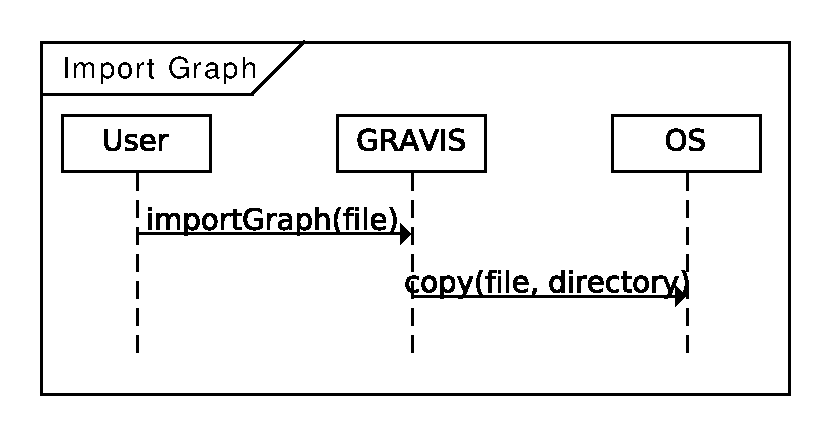
\includegraphics[
% 		    width=\textwidth,
% 		    height=\textheight,
% 		    angle=90,
		    scale=0.5,
		    keepaspectratio=true
	]{diagrams/designmodel/ssd-import-graph.pdf}
    \caption{UC1 Import Graph, System Sequence Diagram}
    \label{fig:import-graph-ssd}
\end{figure}
% \newpage
\begin{figure}[p]% will be the left-side figure
  \begin{leftfullpage}
    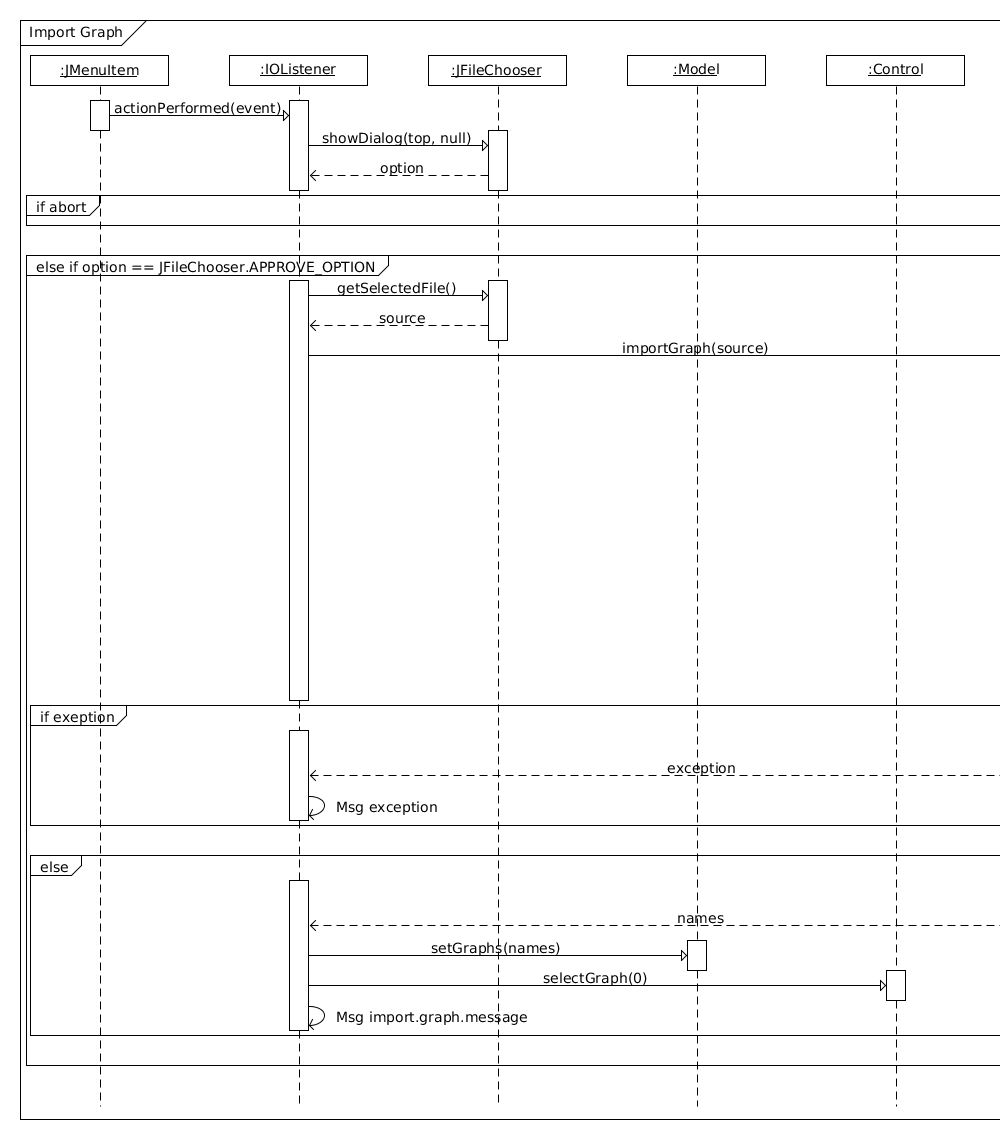
\includegraphics[
% 		    width=\textwidth,
% 		    height=\textheight,
% 		    angle=90,
		    scale=0.42,
% 		    keepaspectratio=true
	]{diagrams/designmodel/sd-import-graph-1-2.png}
    \caption{UC1 Import Graph, Sequence Diagram 1/2}
    \label{fig:import-graph-sd-1}
  \end{leftfullpage}
\end{figure}
\begin{figure}[p]% will be the right-side figure
  \begin{fullpage}
    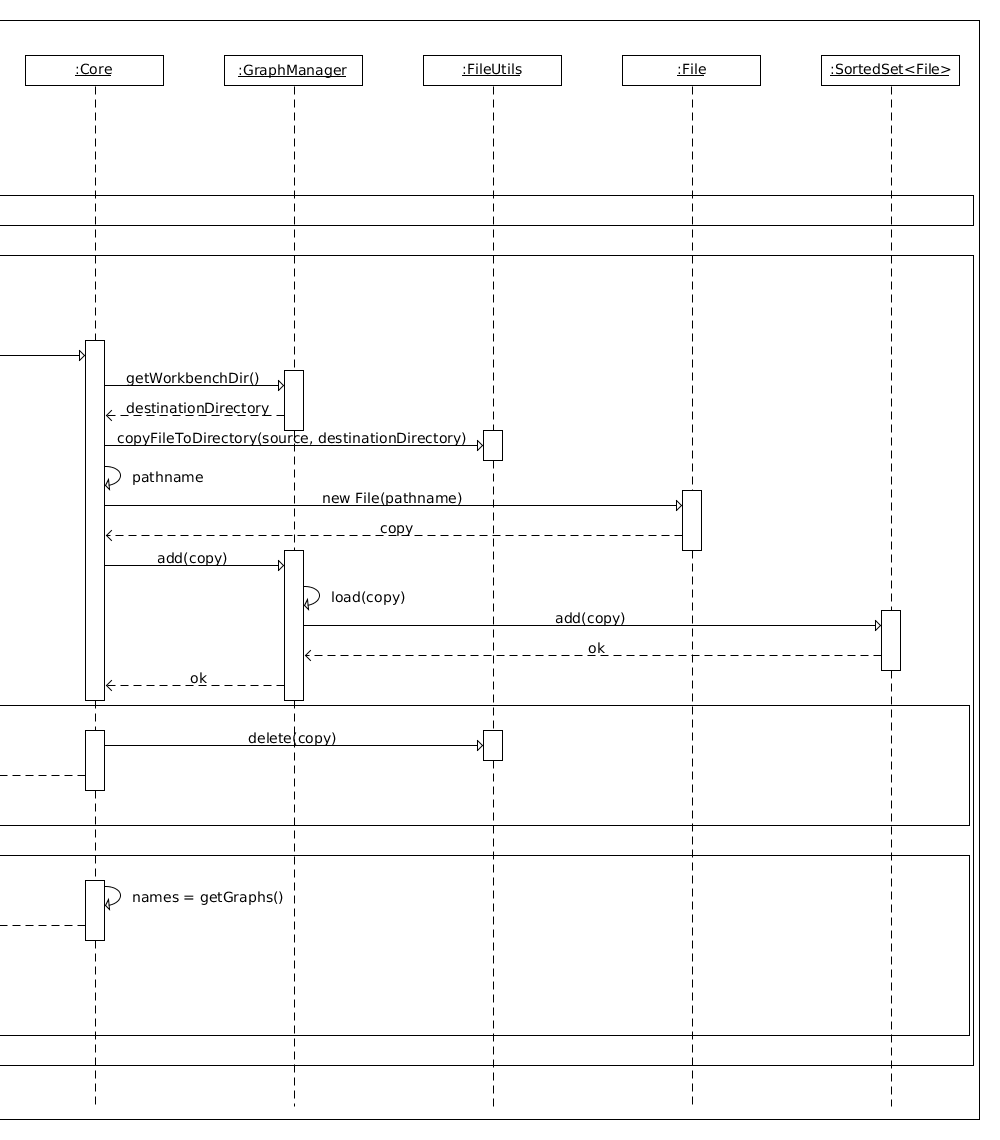
\includegraphics[
% 		    width=\textwidth,
% 		    height=\textheight,
% 		    angle=90,
		    scale=0.42,
% 		    keepaspectratio=true
	]{diagrams/designmodel/sd-import-graph-2-2.png}
    \caption{UC1 Import Graph, Sequence Diagram 2/2}
    \label{fig:import-graph-sd-2}
  \end{fullpage}
\end{figure}
% \newpage
% \begin{figure}[H]
%     \centering
%     \includegraphics[width=\textwidth]{diagrams/designmodel/dcd-import-graph.pdf}
%     \caption{UC1 Import Graph, Design Class Diagram}
%     \label{fig:import-graph-dcd}
% \end{figure}
% ----------------------------------------------------------------------------
% \newpage
% 
\subsubsection{UC2 Import Algorithm}
\begin{figure}[H]
    \centering
    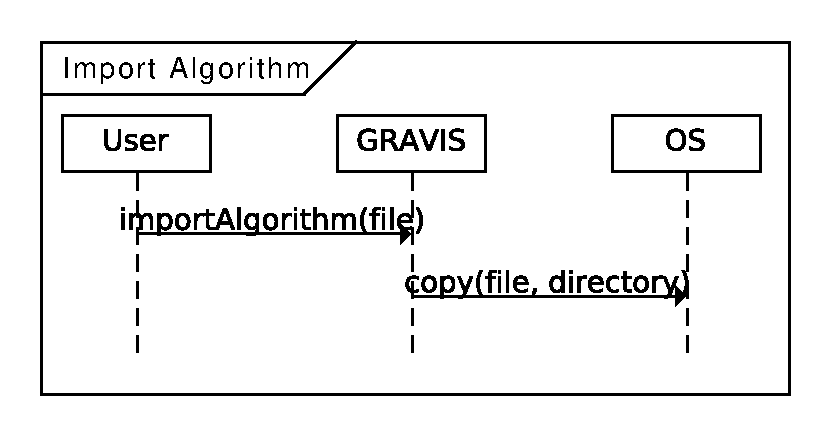
\includegraphics[
% 		    width=\textwidth,
% 		    height=\textheight,
% 		    angle=90,
		    scale=0.5,
		    keepaspectratio=true
      ]{diagrams/designmodel/ssd-import-algorithm.pdf}
    \caption{UC2 Import Algorithm, System Sequence Diagram}
    \label{fig:import-algorithm-ssd}
\end{figure}
% \newpage
\begin{figure}[p]% will be the left-side figure
  \begin{leftfullpage}
    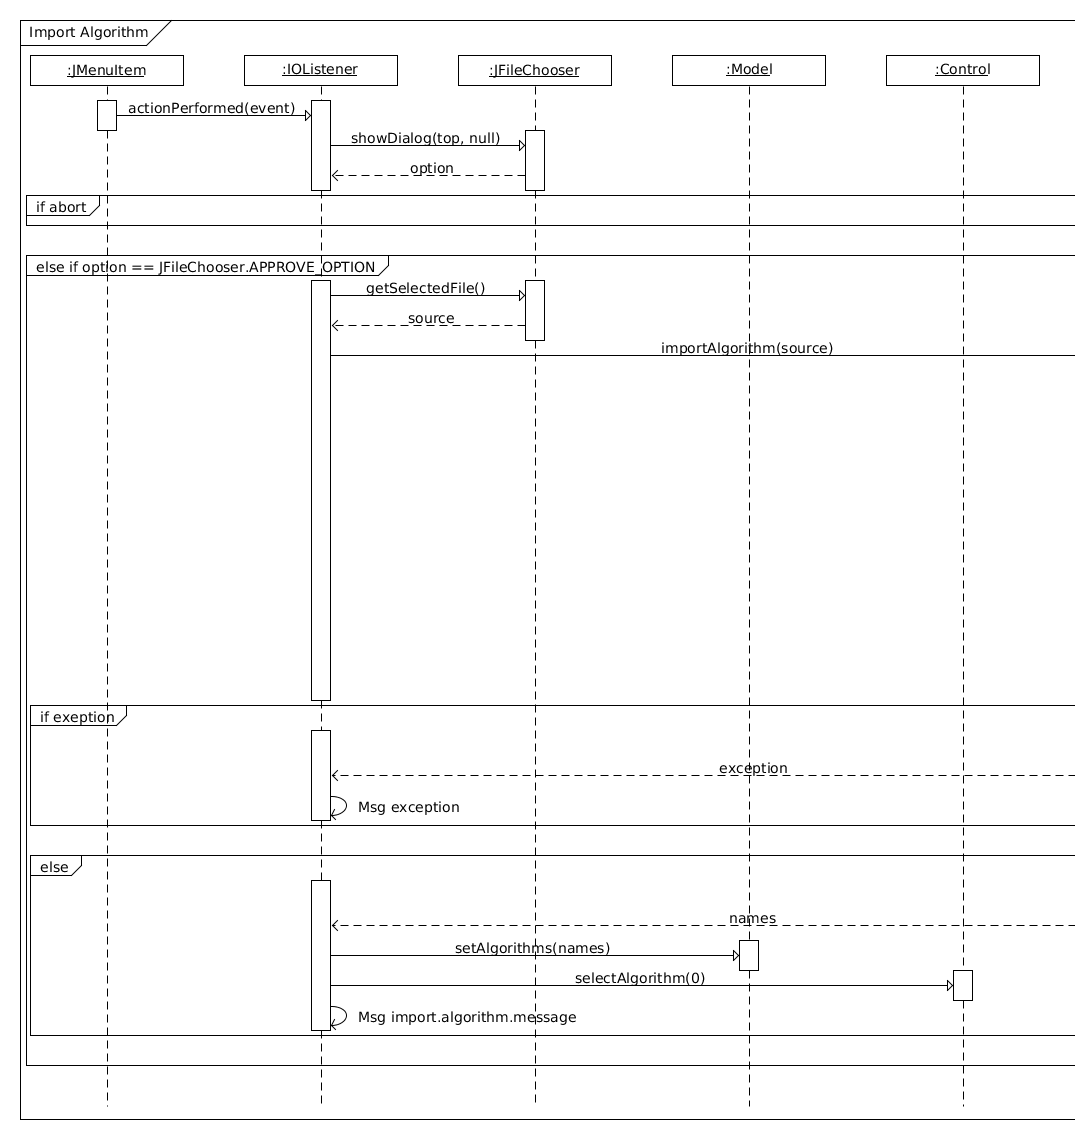
\includegraphics[
% 		    width=\textwidth,
% 		    height=\textheight,
% 		    angle=90,
		    scale=0.42,
% 		    keepaspectratio=true
	]{diagrams/designmodel/sd-import-algorithm-1-2.png}
    \caption{UC2 Import Algorithm, Sequence Diagram 1/2}
    \label{fig:import-algorithm-sd-1}
  \end{leftfullpage}
\end{figure}
\begin{figure}[p]% will be the right-side figure
  \begin{fullpage}
    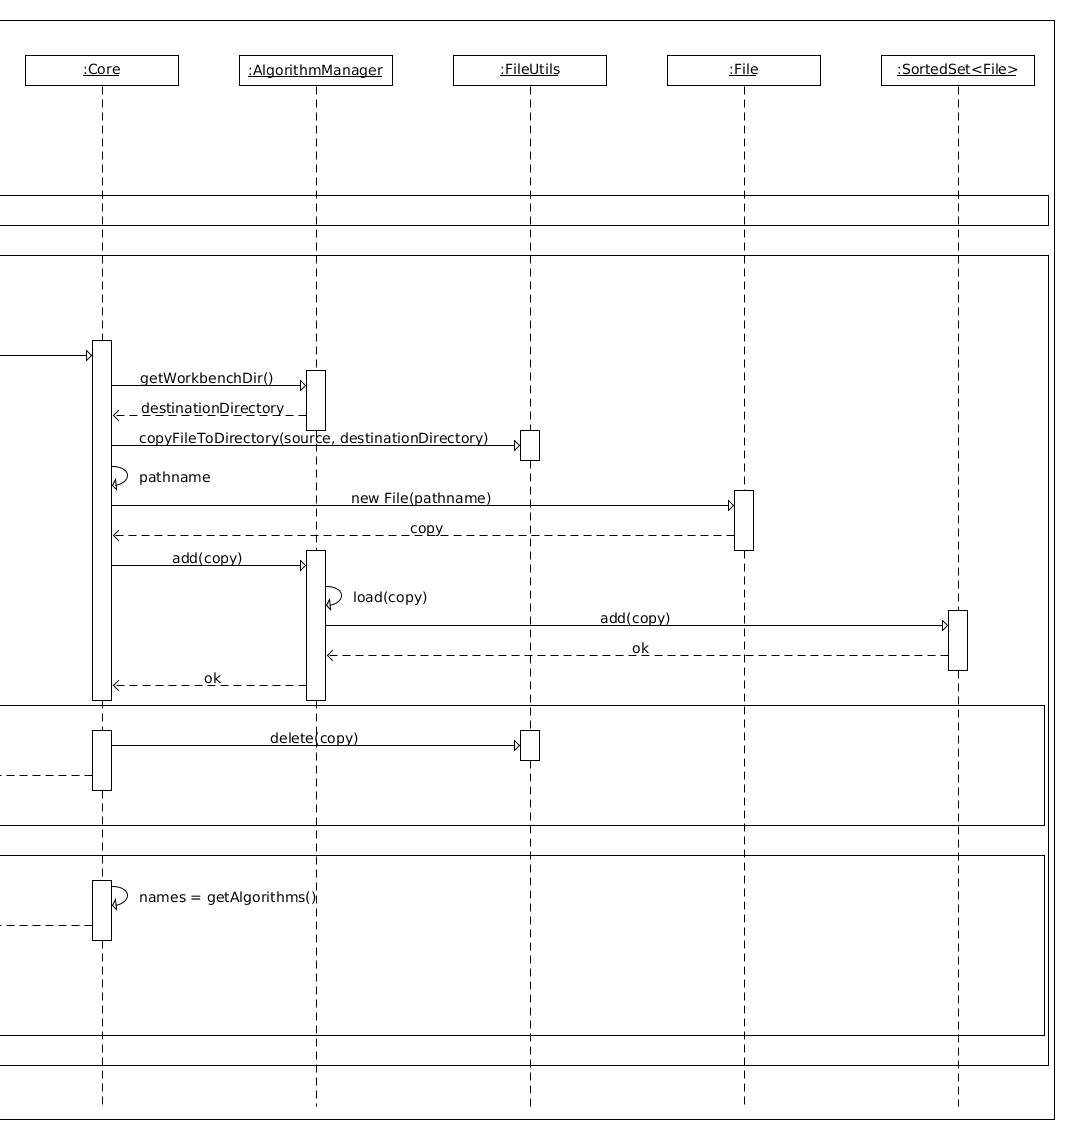
\includegraphics[
% 		    width=\textwidth,
% 		    height=\textheight,
% 		    angle=90,
		    scale=0.42,
% 		    keepaspectratio=true
	]{diagrams/designmodel/sd-import-algorithm-2-2.png}
    \caption{UC2 Import Algorithm, Sequence Diagram 2/2}
    \label{fig:import-algorithm-sd-2}
  \end{fullpage}
\end{figure}
% \newpage
% \begin{figure}[H]
%     \centering
%     \includegraphics[width=\textwidth]{diagrams/designmodel/dcd-import-algorithm.pdf}
%     \caption{UC2 Import Algorithm, Design Class Diagram}
%     \label{fig:import-algorithm-dcd}
% \end{figure}
% ----------------------------------------------------------------------------
% \newpage
% 
\subsubsection{UC3 Delete Graph}
\begin{figure}[H]
    \centering
    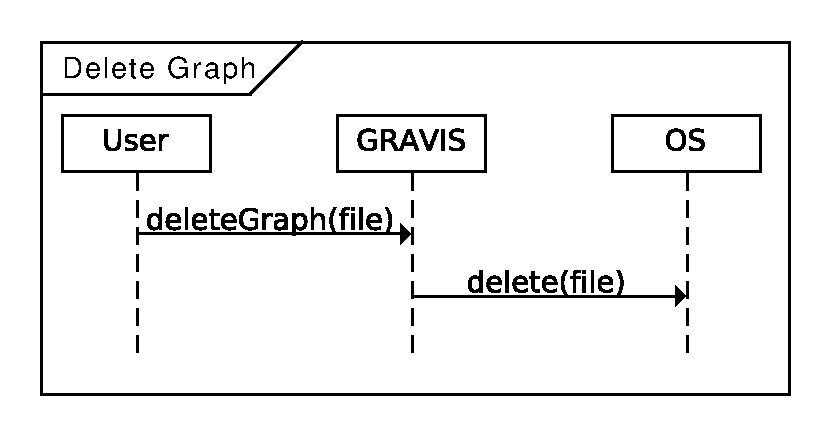
\includegraphics[
% 		    width=\textwidth,
% 		    height=\textheight,
% 		    angle=90,
		    scale=0.5,
		    keepaspectratio=true
      ]{diagrams/designmodel/ssd-delete-graph.pdf}
    \caption{UC3 Delete Graph, System Sequence Diagram}
    \label{fig:delete-graph-ssd}
\end{figure}
% \newpage
\begin{figure}[p]% will be the left-side figure
  \begin{leftfullpage}
    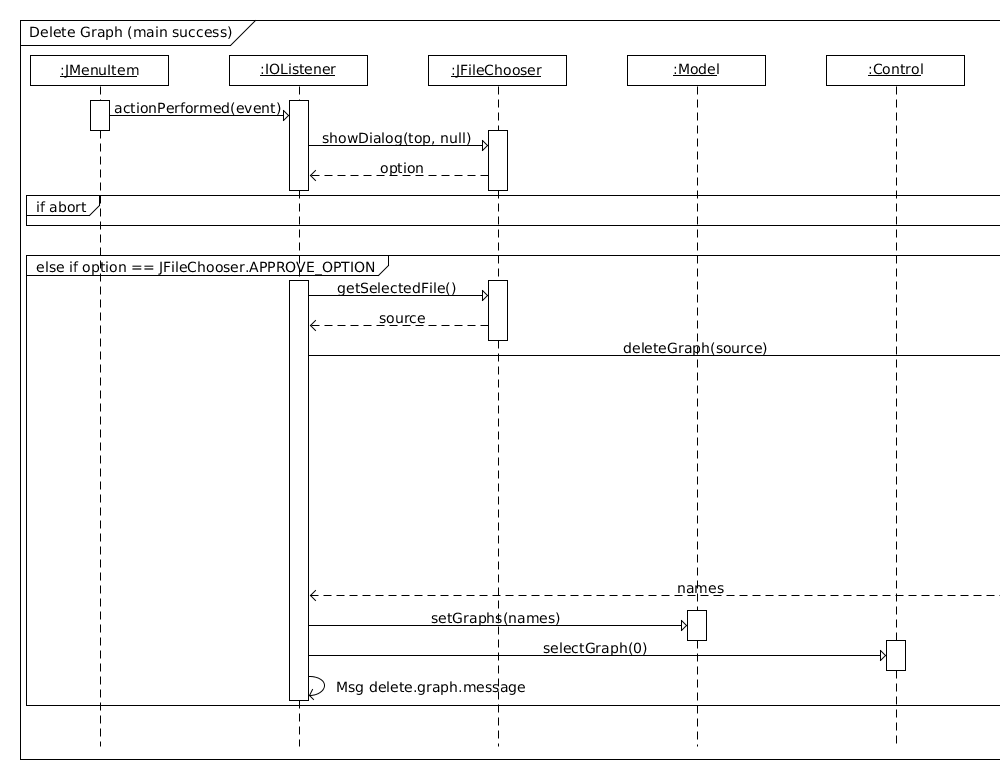
\includegraphics[
% 		    width=\textwidth,
% 		    height=\textheight,
% 		    angle=90,
		    scale=0.42,
% 		    keepaspectratio=true
	]{diagrams/designmodel/sd-delete-graph-1-2.png}
    \caption{UC3 Delete Graph, Sequence Diagram 1/2}
    \label{fig:delete-graph-sd-1}
  \end{leftfullpage}
\end{figure}
\begin{figure}[p]% will be the right-side figure
  \begin{fullpage}
    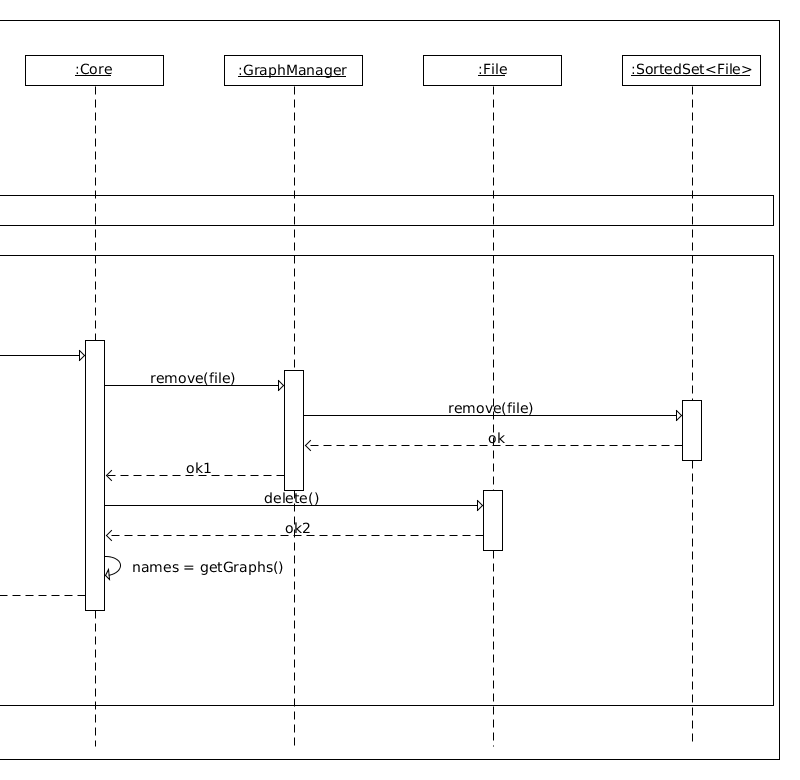
\includegraphics[
% 		    width=\textwidth,
% 		    height=\textheight,
% 		    angle=90,
		    scale=0.42,
% 		    keepaspectratio=true
	]{diagrams/designmodel/sd-delete-graph-2-2.png}
    \caption{UC3 Delete Graph, Sequence Diagram 2/2}
    \label{fig:delete-graph-sd-2}
  \end{fullpage}
\end{figure}
% \newpage
% \begin{figure}[H]
%     \centering
%     \includegraphics[width=\textwidth]{diagrams/designmodel/dcd-delete-graph.pdf}
%     \caption{UC3 Delete Graph, Design Class Diagram}
%     \label{fig:delete-graph-dcd}
% \end{figure}
% ----------------------------------------------------------------------------
% \newpage
% 
\subsubsection{UC4 Delete Algorithm}
\begin{figure}[H]
    \centering
    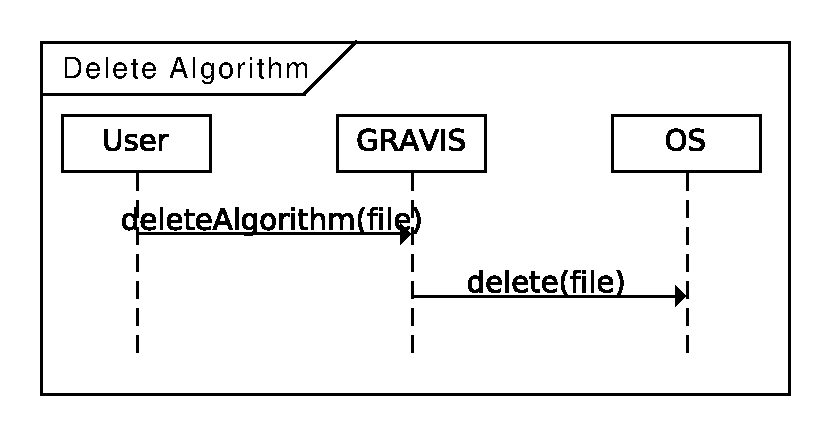
\includegraphics[
% 		    width=\textwidth,
% 		    height=\textheight,
% 		    angle=90,
		    scale=0.5,
		    keepaspectratio=true
      ]{diagrams/designmodel/ssd-delete-algorithm.pdf}
    \caption{UC4 Delete Algorithm, System Sequence Diagram}
    \label{fig:delete-algorithm-ssd}
\end{figure}
% \newpage
\begin{figure}[p]% will be the left-side figure
  \begin{leftfullpage}
    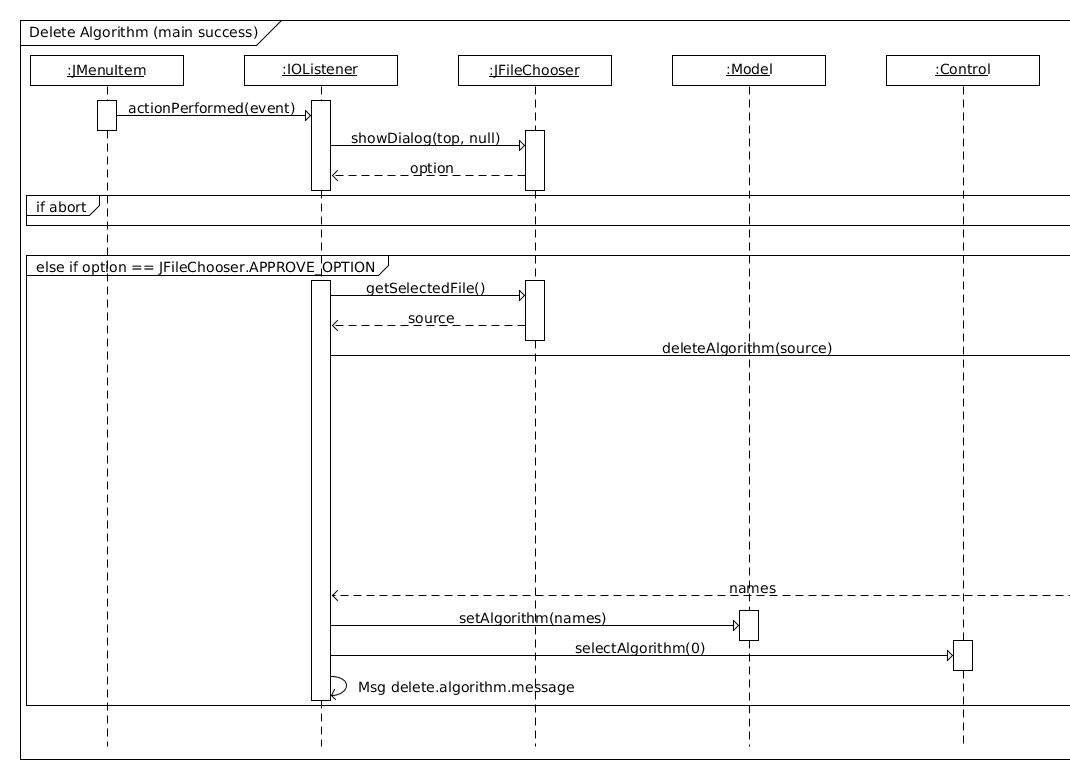
\includegraphics[
% 		    width=\textwidth,
% 		    height=\textheight,
% 		    angle=90,
		    scale=0.42,
% 		    keepaspectratio=true
	]{diagrams/designmodel/sd-delete-algorithm-1-2.png}
    \caption{UC4 Delete Algorithm, Sequence Diagram 1/2}
    \label{fig:delete-algorithm-sd-1}
  \end{leftfullpage}
\end{figure}
\begin{figure}[p]% will be the right-side figure
  \begin{fullpage}
    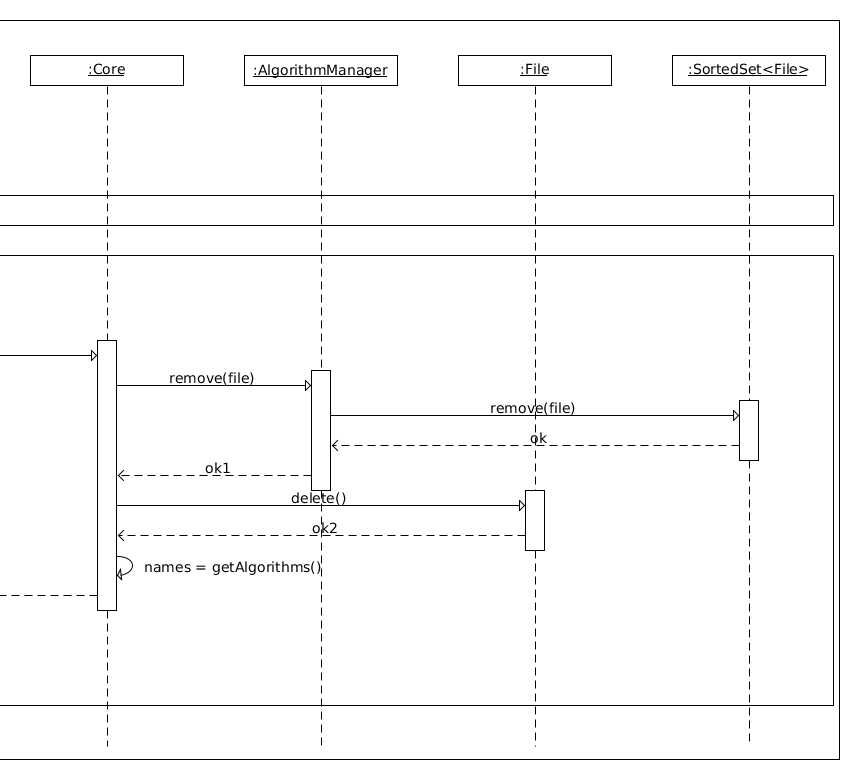
\includegraphics[
% 		    width=\textwidth,
% 		    height=\textheight,
% 		    angle=90,
		    scale=0.42,
% 		    keepaspectratio=true
	]{diagrams/designmodel/sd-delete-algorithm-2-2.png}
    \caption{UC4 Delete Algorithm, Sequence Diagram 2/2}
    \label{fig:delete-algorithm-sd-2}
  \end{fullpage}
\end{figure}
% \newpage
% \begin{figure}[H]
%     \centering
%     \includegraphics[width=\textwidth]{diagrams/designmodel/dcd-delete-algorithm.pdf}
%     \caption{UC4 Delete Algorithm, Design Class Diagram}
%     \label{fig:delete-algorithm-dcd}
% \end{figure}
% ----------------------------------------------------------------------------
% \newpage
% 
\subsubsection{Parameter Controller}
\begin{figure}[H]
    \centering
    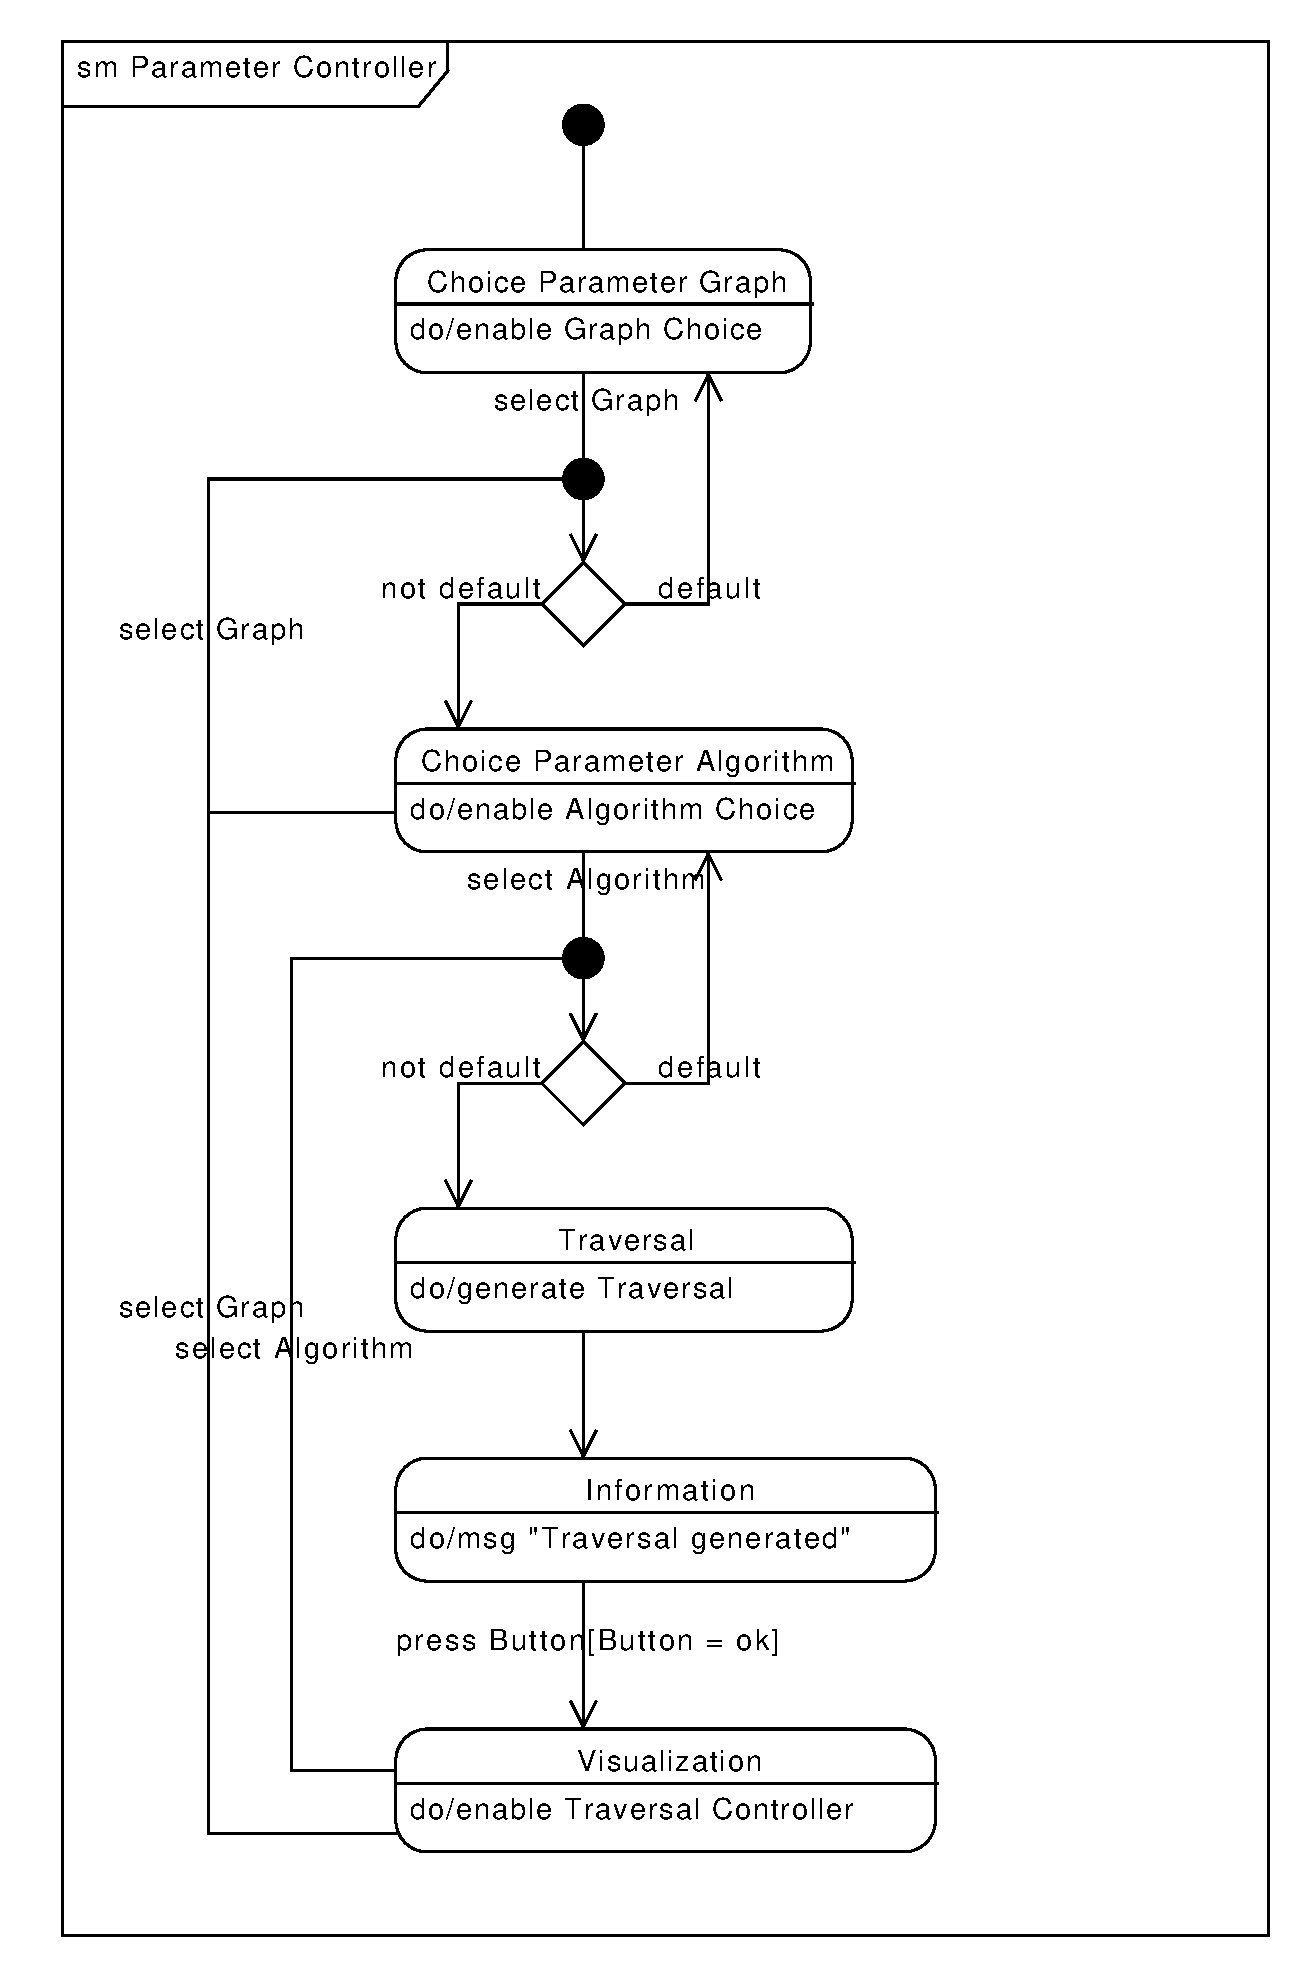
\includegraphics[
% 		    width=\textwidth,
% 		    height=\textheight,
% 		    angle=90,
		    scale=0.6,
		    keepaspectratio=true
    ]{diagrams/designmodel/sm-parameter-controller.pdf}
    \caption{Parameter Controller, State Diagram}
    \label{fig:parameter-controller-sm}
\end{figure}
% ----------------------------------------------------------------------------
% \newpage
% 
\subsubsection{UC5 Select Graph}
\begin{figure}[H]
    \centering
    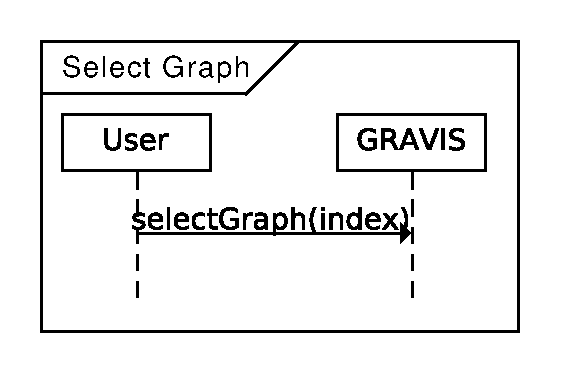
\includegraphics[
% 		    width=\textwidth,
% 		    height=\textheight,
% 		    angle=90,
		    scale=0.5,
		    keepaspectratio=true
      ]{diagrams/designmodel/ssd-select-graph.pdf}
    \caption{UC5 Select Graph, System Sequence Diagram}
    \label{fig:select-graph-ssd}
\end{figure}
% \newpage
% \begin{figure}[p]% will be the left-side figure
%   \begin{leftfullpage}
% %     \includegraphics[
% % 		    width=\textwidth,
% % 		    height=\textheight,
% % 		    angle=90,
% 		    scale=0.42,
% 		    keepaspectratio=true
% 	]{diagrams/designmodel/sd-select-graph-1-2.png}
%     \caption{UC5 Select Graph, Sequence Diagram 1/2}
%     \label{fig:select-graph-sd-1}
%   \end{leftfullpage}
% \end{figure}
% \begin{figure}[p]% will be the right-side figure
%   \begin{fullpage}
% %     \includegraphics[
% % 		    width=\textwidth,
% % 		    height=\textheight,
% % 		    angle=90,
% 		    scale=0.42,
% 		    keepaspectratio=true
% 	]{diagrams/designmodel/sd-select-graph-2-2.png}
%     \caption{UC5 Select Graph, Sequence Diagram 2/2}
%     \label{fig:select-graph-sd-2}
%   \end{fullpage}
% \end{figure}
% \newpage
% \begin{figure}[H]
%     \centering
%     \includegraphics[width=\textwidth]{diagrams/designmodel/dcd-select-graph.pdf}
%     \caption{UC5 Select Graph, Design Class Diagram}
%     \label{fig:select-graph-dcd}
% \end{figure}
% ----------------------------------------------------------------------------
% \newpage
% 
\subsubsection{UC6 Select Algorithm}
\begin{figure}[H]
    \centering
    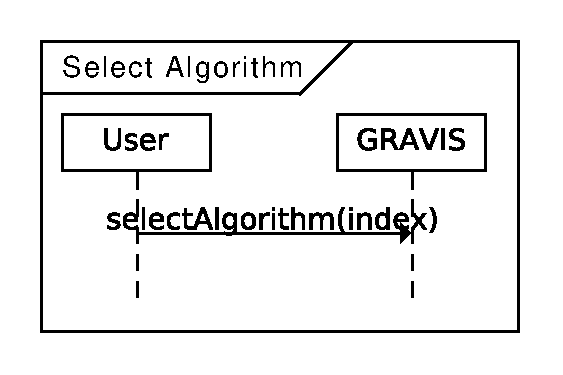
\includegraphics[
% 		    width=\textwidth,
% 		    height=\textheight,
% 		    angle=90,
		    scale=0.5,
		    keepaspectratio=true
      ]{diagrams/designmodel/ssd-select-algorithm.pdf}
    \caption{UC6 Select Algorithm, System Sequence Diagram}
    \label{fig:select-algorithm-ssd}
\end{figure}
% \newpage
% \begin{figure}[p]% will be the left-side figure
%   \begin{leftfullpage}
% %     \includegraphics[
% % 		    width=\textwidth,
% % 		    height=\textheight,
% % 		    angle=90,
% 		    scale=0.42,
% 		    keepaspectratio=true
% 	]{diagrams/designmodel/sd-select-algorithm-1-2.png}
%     \caption{UC6 Select Algorithm, Sequence Diagram 1/2}
%     \label{fig:select-algorithm-sd-1}
%   \end{leftfullpage}
% \end{figure}
% \begin{figure}[p]% will be the right-side figure
%   \begin{fullpage}
% %     \includegraphics[
% % 		    width=\textwidth,
% % 		    height=\textheight,
% % 		    angle=90,
% 		    scale=0.42,
% 		    keepaspectratio=true
% 	]{diagrams/designmodel/sd-select-algorithm-2-2.png}
%     \caption{UC6 Select Algorithm, Sequence Diagram 2/2}
%     \label{fig:select-algorithm-sd-2}
%   \end{fullpage}
% \end{figure}
% \newpage
% \begin{figure}[H]
%     \centering
%     \includegraphics[width=\textwidth]{diagrams/designmodel/dcd-select-algorithm.pdf}
%     \caption{UC6 Select Algorithm, Design Class Diagram}
%     \label{fig:select-algorithm-dcd}
% \end{figure}
% ----------------------------------------------------------------------------
% \newpage
% 
\subsubsection{Traversal Controller}
\begin{figure}[H]
    \centering
    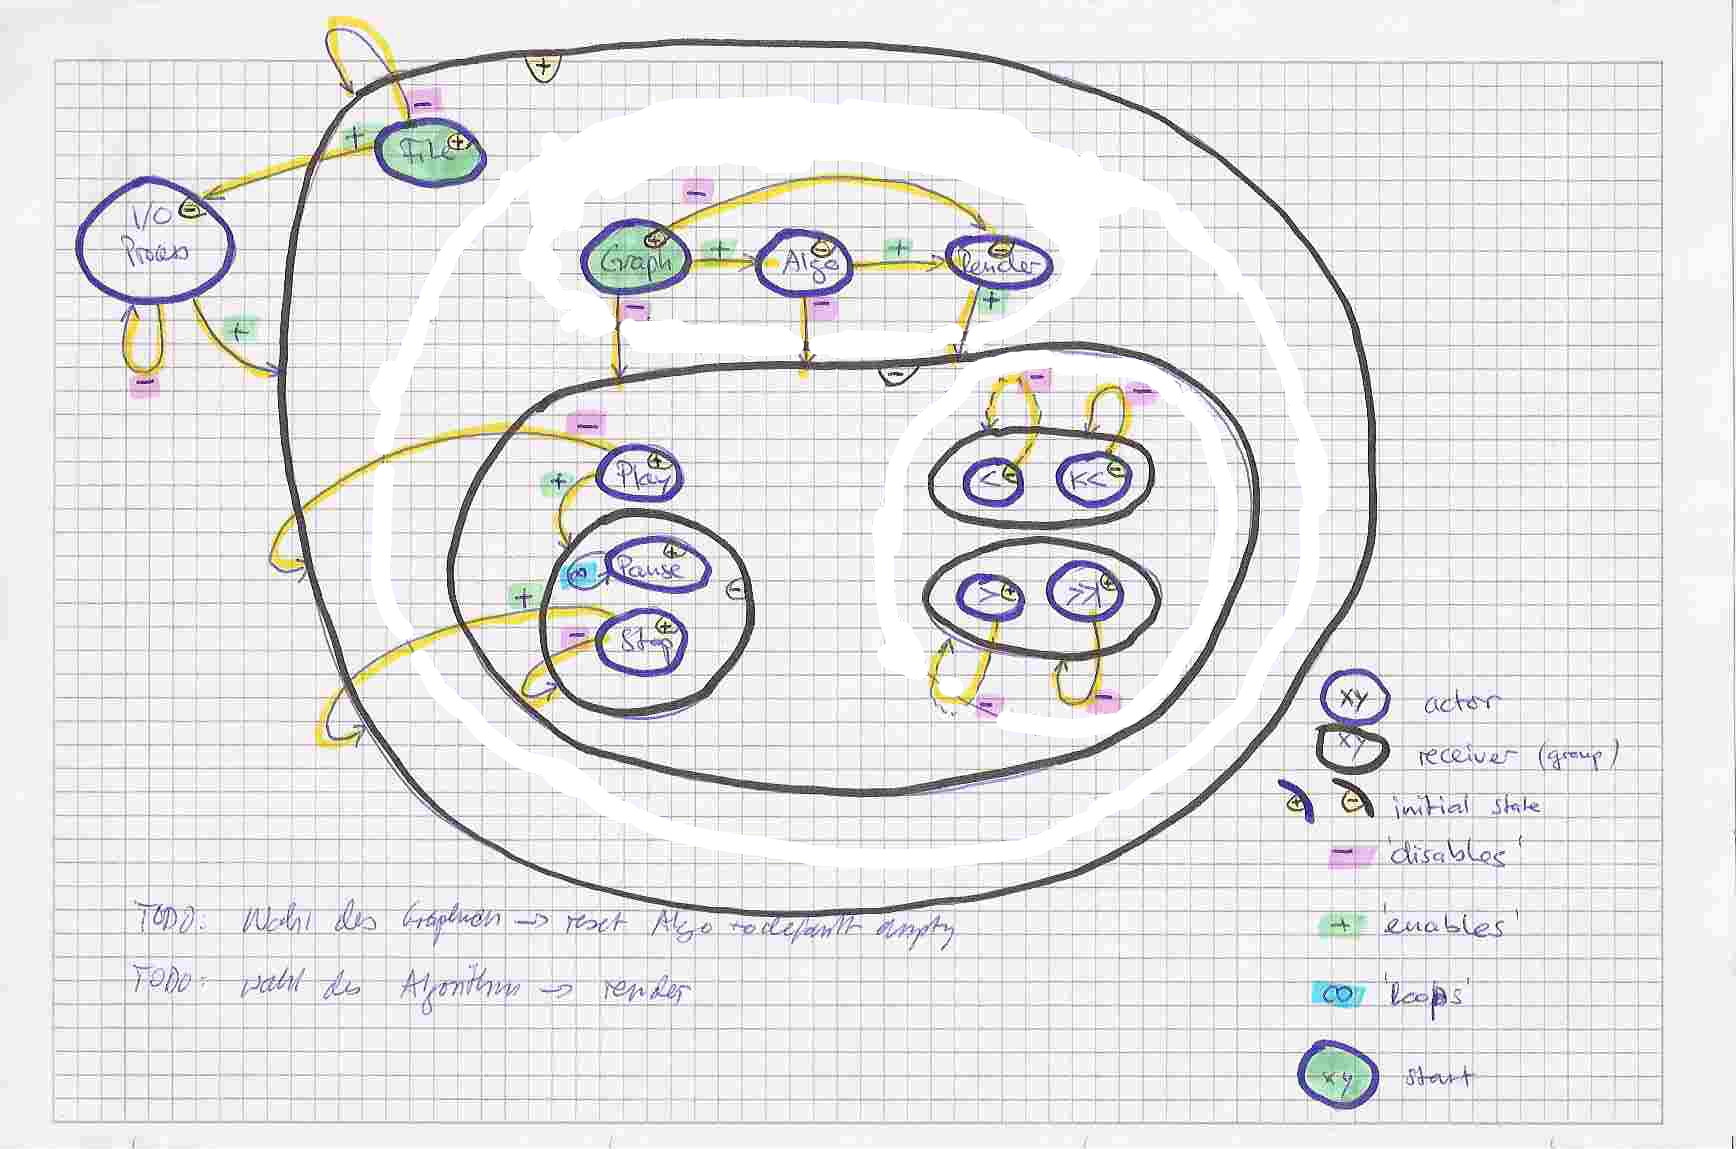
\includegraphics[
		    width=\textwidth,
% 		    height=\textheight,
% 		    angle=90,
		    scale=0.5,
		    keepaspectratio=true
    ]{diagrams/designmodel/sm-traversal-controller_draft_v2.jpeg}
    \caption{Traversal Controller, State Diagram}
    \label{fig:traversal-controller-sm}
\end{figure}